\documentclass[conference,onecolumn,11pt]{IEEEtran}
\IEEEoverridecommandlockouts
% The preceding line is only needed to identify funding in the first footnote. If that is unneeded, please comment it out.
\usepackage{amsmath,amssymb,amsfonts}
\usepackage{algorithmic}
\usepackage{graphicx}
\usepackage{textcomp}
\usepackage{xcolor}
\usepackage{hyperref}
\usepackage{booktabs} % for tables
\usepackage{biblatex}
\addbibresource{cite.bib}


\def\BibTeX{{\rm B\kern-.05em{\sc i\kern-.025em b}\kern-.08em
    T\kern-.1667em\lower.7ex\hbox{E}\kern-.125emX}}
\begin{document}

\title{Predicting Stock Market Volatility with Time Series Models\\
}

\author{\IEEEauthorblockN{1\textsuperscript{st} Xu Hao}
\IEEEauthorblockA{\textit{Department of Mathematics \& Statistics} \\
\textit{Thompson Rivers University}\\
Kamloops, Canada \\
xuh23@mytru.ca}
\and
\IEEEauthorblockN{2\textsuperscript{nd} Mulk Waqar Ul}
\IEEEauthorblockA{\textit{Department of Mathematics \& Statistics} \\
\textit{Thompson Rivers University}\\
Kamloops, Canada \\
mulkw22@mytru.ca}
}

\maketitle

\begin{abstract}
Predicting stock market movements is a significant challenge for traders, investors, and businesses, yet it can be highly profitable with precise forecasts. Achieving accurate predictions is crucial, particularly given the volatile, nonlinear, and unpredictable nature of the stock market. In this paper we are predicting stock prices of Apple using two machine learning algorithms - Linear Regression and Autoregressive Integrated Moving Average (ARIMA) by comparing their forecasting performances. The data is collected from Yahoo Finance and Google Trends and the analysis spans a period of eight years, from April 1st, 2016, to March 31st, 2024. The performance of the models are evaluated by root mean squared error (RMSE), mean squared error (MSE) and R-squared (R2). The findings of this study demonstrate that Simple Linear Regression is not well-suited for time series data analysis, whereas ARIMA presents distinct advantages in forecasting stock prices.

\end{abstract}

\begin{IEEEkeywords}
Forecasting, Stock Prices, Machine Learning, Autoregression, Linear Regression. 
\end{IEEEkeywords}

\section{Introduction}
A stock signifies an investment representing ownership in a company. The total ownership of a company is divided into shares, with each share representing an equal portion of the business. The stock market functions as a marketplace where individuals can purchase shares of stock. Analogous to various other markets like grocery stores or farmers’ markets, where multiple vendors gather to sell their products, the stock market serves as a central hub for trading securities. Similarly to a farmers’ market where different farmers offer their produce, customers have the opportunity to explore various investment options and make purchases according to their preferences. In essence, the stock market operates similarly to these markets, acting as a centralized venue where buyers and sellers converge to trade stocks and other investment instruments, including mutual funds, which pool together multiple stocks. However, unlike a single market, the stock market comprises several smaller markets known as stock exchanges.
Utilizing machine learning algorithms for stock price prediction aids in uncovering the potential future value of company stocks and other financial assets traded on various exchanges. The fundamental objective of predicting stock prices is to attain substantial profits. However, forecasting the performance of the stock market is a formidable challenge. Several factors come into play in this prediction process, encompassing both tangible and psychological elements, rational and irrational behaviors, among others.
The interaction of these diverse factors renders share prices highly dynamic and volatile, thereby posing significant hurdles to achieving precise predictions with a high degree of accuracy.


\subsection*{Linear Regression}

Linear regression is a statistical method used to model the relationship between a dependent variable and one or more independent variables by fitting a linear equation to observed data. In essence, it seeks to determine the best-fitting straight line through the data points. The goal is to find the coefficients of the linear equation that minimize the difference between the observed and predicted values of the dependent variable. Linear regression is widely employed for prediction and forecasting tasks, as well as for understanding the relationships between variables in a dataset.

$Y = \beta_0+\beta_1 x_1 + \beta_2 x_2 + \ldots+\beta_n x_n + \epsilon$
y represents the dependent variable, x1, x2, ..., xn represents the independent variables, $\beta_0,\beta_1,\beta_2,\ldots,\beta_n$ represents the coefficients associated with each independent variable, and n is the number of independent variables. $\epsilon$represents the error term, which captures the difference between the observed and predicted values of the dependent variable.


\subsection*{ARIMA}

ARIMA, or AutoRegressive Integrated Moving Average, is a forecasting algorithm grounded in the principle that historical values of a time series can offer insights into future trends. Belonging to a class of models renowned for elucidating time series behavior through its own past data, including lags and lagged forecast errors, ARIMA excels in predicting forthcoming values. It is particularly applicable to time series datasets exhibiting discernible patterns rather than random noise. ARIMA entails three key parameters: p, d, and q. The parameter p denotes the number of autoregressive terms or lag observations, providing lagged data points. d signifies the degree of differencing, indicating the number of times lagged indicators have been subtracted to achieve data stationarity. q represents the number of forecast errors in the model, akin to the size of the moving average window. These parameters, integers by nature, are pivotal in defining the ARIMA model's functionality and can take a value of 0, implying their exclusion from the model. Consequently, ARIMA can transform into various models: ARMA (p=0, d=0), AR (p$>$0, d=0, q=0), and MA (p=0, d=0, q$>$0). ARIMA models are denoted by their parameter combinations, such as ARIMA(1, 0, 0) for the first-order autoregressive model or ARIMA(0, 1, 0) for the random walk model. Once the parameters are set, the ARIMA model estimates coefficients $\alpha$ and $\theta$, utilizing past data points to forecast future values.

\section{Literature review}

Many researchers have done their studies in predicting stock prices using similar  machine learning models, some of them are discussed below. \\
In 2011 Selene Yue Xu wrote a paper on predicting stock prices for Apple Inc. Her paper focuses on stock price forecasting by combining conventional time series analysis with information from Yahoo Finance and Google Trend. It aims to predict weekly changes in stock price, particularly focusing on Apple Inc. stock. Her study records important news/events related to Apple Inc. over a five-year span and uses the weekly Google trend index values to measure the magnitude of these events. The data includes weekly stock prices of Apple Inc. and key developments from Yahoo Finance, while her analysis involves applying the ARIMA model, differencing the data, and regressing stock price changes on news values. The paper also presents an algorithm for computing the value of news at a certain time, simulating the impact of news on stock prices. Her analysis reveals a significant correlation between the changes in weekly stock prices and the values of important news/events computed from the Google trend website.\\



\section{Data}
Data used for this paper is taken from Yahoo finance and Google Trend data. As we are only focused on Apple stocks data, we got the data only for Apple which ranges from April 1st, 2016 till March 31st, 2024. It consists of 6 independent variables and one response variable. The adjusted close price is a variable which we are using both as an independent and dependent variable. Table 1 shows statistics of the dataset that is used for training and testing.

\begin{table}[htbp]
    \centering
    \caption{Dataset Splitting}
    \begin{tabular}{@{}rlllll@{}}
        \toprule
         && \textbf{Dataset} & \textbf{Training} & \textbf{Validation} & \textbf{Testing} \\
        \midrule
        \textbf{Time Interval} &(Start) & 04-01-2016 & 04-01-2016 & 01-02-2021 & 07-01-2023\\
        &(End)& 03-31-2024 & 01-01-2021 & 06-30-2023 & 03-31-2024\\
  
        \bottomrule
    \end{tabular}
    \label{tab:GFS}
\end{table}

\begin{figure}[htpb]
	\centering
	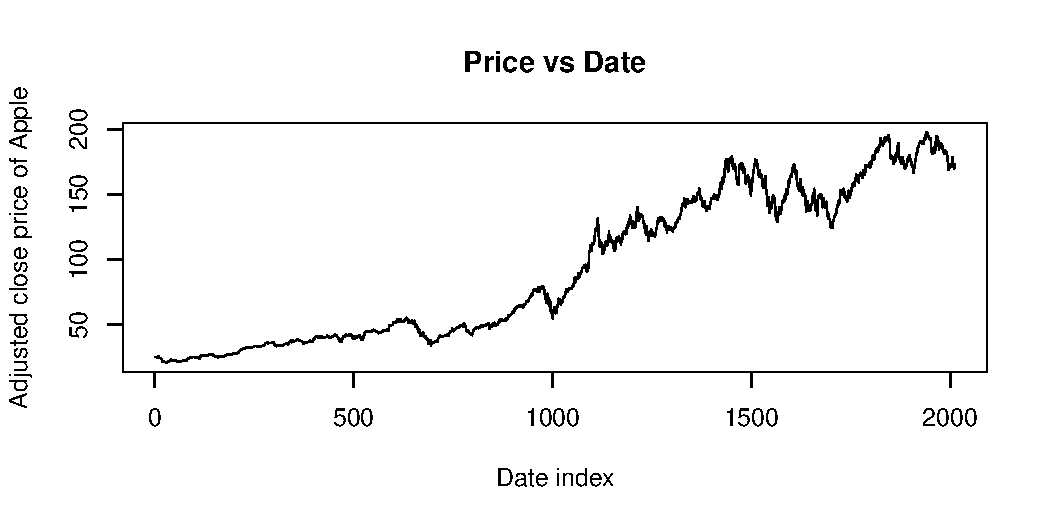
\includegraphics[width=0.8\textwidth]{pic/Price_vs_Date.pdf}
	\caption{}
	\label{fig:price}
\end{figure}

\begin{figure}[htpb]
	\centering
	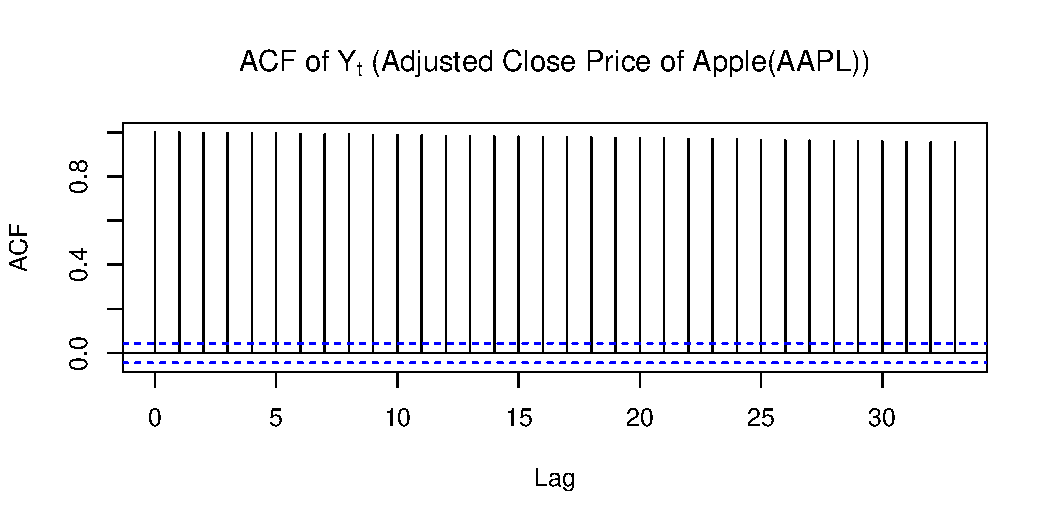
\includegraphics[width=0.8\textwidth]{pic/ACF_AdjClosed.pdf}
	\caption{}
	\label{fig:acf1}
\end{figure}

\begin{figure}[htpb]
	\centering
	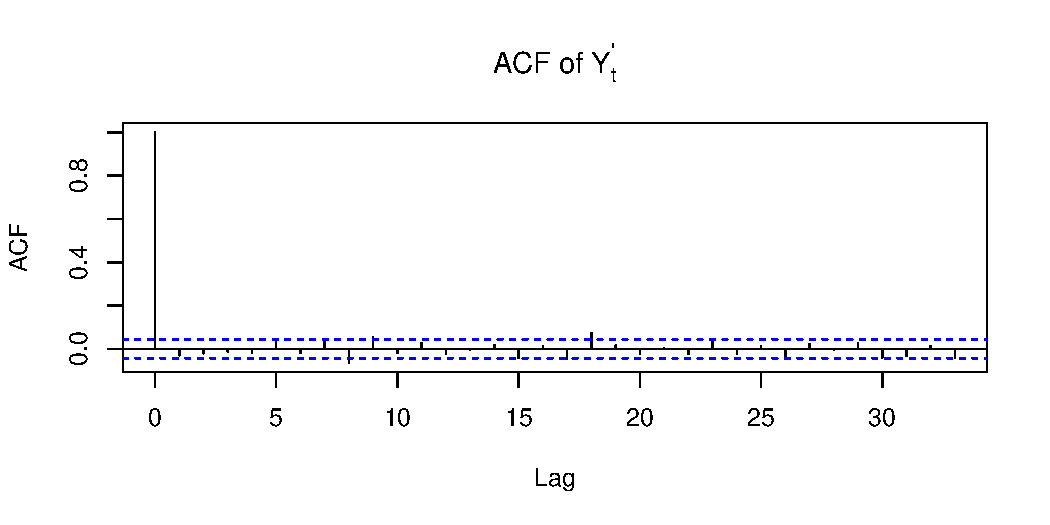
\includegraphics[width=0.8\textwidth]{pic/ACF_dAdjClosed.pdf}
	\caption{}
	\label{fig:acf2}
\end{figure}

Plot the graphs of $\sqrt{y_t}-\sqrt{y_{t-1}}$ (as shown in Fig.~\ref{fig:dsqrt}) and $\ln(y_t)-\ln(y_{t-1})$ (as shown in Fig.~\ref{fig:dlog}) to compare. 

\begin{figure}[htpb]
	\centering
	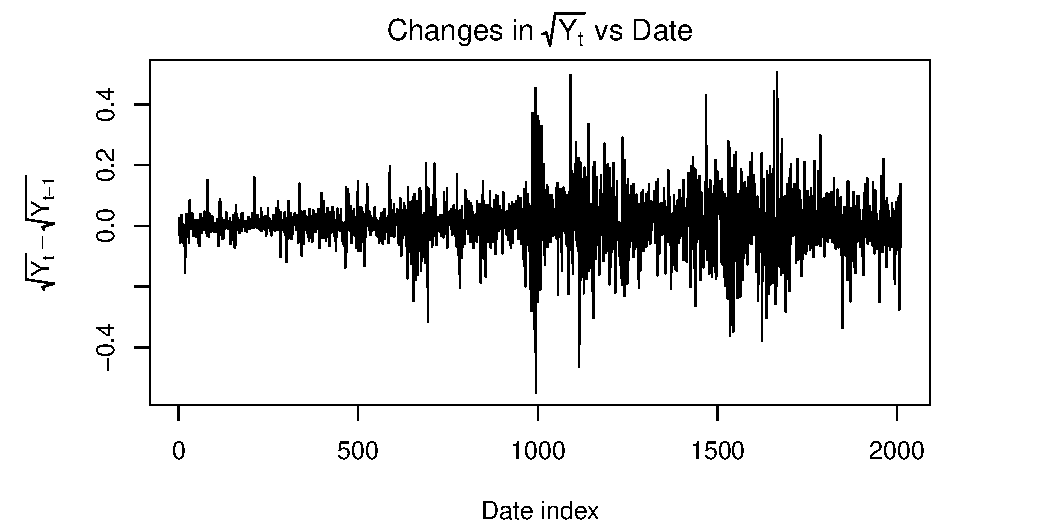
\includegraphics[width=0.8\textwidth]{pic/Sqrt_AdjClosed.pdf}
	\caption{}
	\label{fig:dsqrt}
\end{figure}

\begin{figure}[htpb]
	\centering
	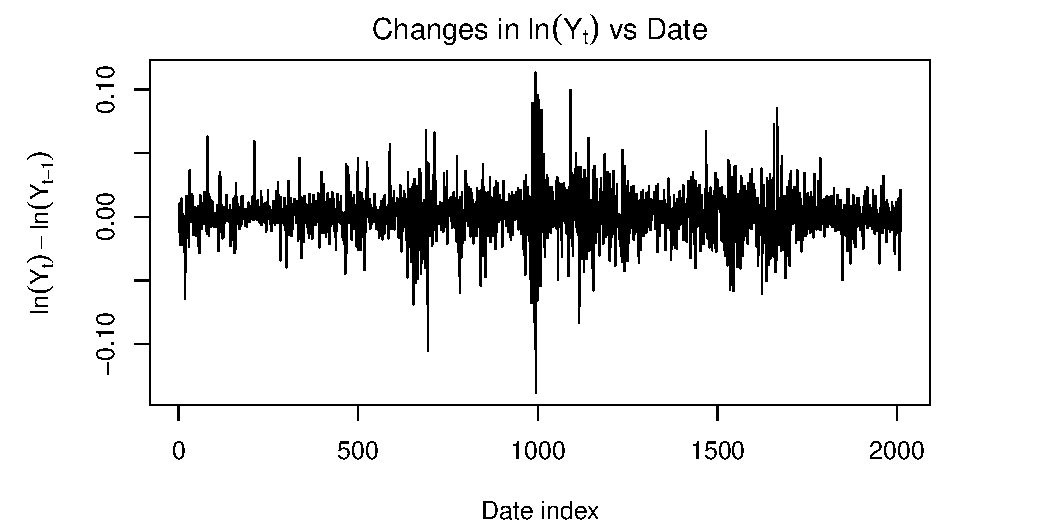
\includegraphics[width=0.8\textwidth]{pic/log_AdjClosed.pdf}
	\caption{}
	\label{fig:dlog}
\end{figure}


\section{Method}

\subsection*{Autoregression with one variable}\label{mod1}

We use $y_{t}$ to represent the adjusted close price of Apple stock.
$y^{'}_{t} = \ln(y_{t})-\ln(y_{t-1}) = \ln(\frac{y_{t}}{y_{t-1}})$ represent the first difference of log of $y_{t}$.


Our AR($p$) model is defined as follows:

\[
y^{'}_{t} = c + \phi_{1}y^{'}_{t-1} + \phi_{2}y^{'}_{t-2} + \dots + \phi_{p}y^{'}_{t-p} + \varepsilon_{t},
\]

The predicted value for $y_t$ is calculated as follows:

\[
\hat{y}_t = \exp\{c + \phi_{1}y^{'}_{t-1} + \phi_{2}y^{'}_{t-2} + \dots + \phi_{p}y^{'}_{t-p}\}\cdot y_{t-1}
\]

\subsection*{Autoregression with multiple variables}
\label{mod2}

From Google trends, we get the interest over time of keywords ``Apple Watch", ``MacBook", ``AirPods", ``iPad", ``iPhone", represented by variable $y_{3,t},y_{4,t},y_{5,t},y_{6,t},y_{7,t}$ respectively. Also, we take the volume of the apple stock represented by variable $y_{2,t}$, the first difference of the adjusted close price of Apple stock as $y_{1,t}$ (which is also $y^{'}_t$ scenario). $\mathbf{y}_t = (y_{1,t},y_{2,t},y_{3,t},y_{4,t},y_{5,t},y_{6,t},y_{7,t})$.

We define our Vector Auto-Regressive(VAR) model as follows:

\[
y^{'}_t = \boldsymbol{\phi}_1\mathbf{y}_{t-1}^T+\ldots+\boldsymbol{\phi}_p\mathbf{y}_{t-p}^T+\epsilon_t
\]

where $\boldsymbol{\phi}_i$ are $(1\times7)$ coefficient vector for $i=1,\ldots,p$.




\section{Results}
\section{Discussion and/or Conclusion}

\section{Writing styles}

\begin{itemize}
\item Font: Times New Roman. The size of the font for the main body text must be 11 pt. 
\item One column. 
\item Single line spacing. 
\item Citations/references are to be done in Vancouver style. Citations are marked by a number in square brackets [1], which refers to a numbered reference in the references section.\cite{Xu2018},\cite{Khanderwal2021},\cite{Vijh2020}
\item Sections should be clearly titled and numbered. 
\end{itemize}

\subsection{Equations}
Number equations consecutively. To make your 
equations more compact, you may use the solidus (~/~), the exp function, or 
appropriate exponents. Italicize Roman symbols for quantities and variables, 
but not Greek symbols. Use a long dash rather than a hyphen for a minus 
sign. Punctuate equations with commas or periods when they are part of a 
sentence, as in:
\begin{equation}
a+b=\gamma\label{eq}
\end{equation}

Be sure that the 
symbols in your equation have been defined before or immediately following 
the equation. Use ``\eqref{eq}'', not ``Eq.~\eqref{eq}'' or ``equation \eqref{eq}'', except at 
the beginning of a sentence: ``Equation \eqref{eq} is . . .''

\printbibliography

\vspace{12pt}
\end{document}
